\documentclass[letterpaper,10pt]{article}

%\setlength{\parindent}{0in}
%\usepackage{fullpage} 
\usepackage{amsmath}
\usepackage{amssymb}
\usepackage{enumerate}
\usepackage{graphicx}
\usepackage[table]{xcolor}
\usepackage{dcolumn}
\usepackage[english]{babel}
\oddsidemargin 0.0in
\textwidth 6.5in
\newcolumntype{.}{D{.}{.}{-1}}
\newcommand*{\myalign}[2]{\multicolumn{1}{#1}{#2}}
% Alter some LaTeX defaults for better treatment of figures:
    % See p.105 of "TeX Unbound" for suggested values.
    % See pp. 199-200 of Lamport's "LaTeX" book for details.
    %   General parameters, for ALL pages:
    \renewcommand{\topfraction}{0.9}	% max fraction of floats at top
    \renewcommand{\bottomfraction}{0.8}	% max fraction of floats at bottom
    %   Parameters for TEXT pages (not float pages):
    \setcounter{topnumber}{2}
    \setcounter{bottomnumber}{2}
    \setcounter{totalnumber}{4}     % 2 may work better
    \setcounter{dbltopnumber}{2}    % for 2-column pages
    \renewcommand{\dbltopfraction}{0.9}	% fit big float above 2-col. text
    \renewcommand{\textfraction}{0.07}	% allow minimal text w. figs
    %   Parameters for FLOAT pages (not text pages):
    \renewcommand{\floatpagefraction}{0.7}	% require fuller float pages
	% N.B.: floatpagefraction MUST be less than topfraction !!
    \renewcommand{\dblfloatpagefraction}{0.7}	% require fuller float pages

%Repeat the example shown in the output analysis classes, except use Server utilization as your metric. Steps to complete:
%
%    Use an appropriate warm-up period if warranted.  Tell me what time you used and justify why you think you should have a warm up period (or not).
%    Measure mean server utilization for each of 50 replications.
%    Export the data to the statistical package of your choice
%    Repeat this step 3 times
%    Produce a confidence interval for one column of data
%    Produce a 2-sample t test for two columns of data
%    Produce an ANOVA comparing all three columns of data
%    In Extend, change the inter-arrival time from Exponential to Triangular (2,3,4) and generate 50 new observations - note that the Triangular distribution is usually designated by specifying the (minimum, most likely, maximum) values - in ExtendSim, however, the Triangular dialogue takes input in the order (minimum, maximum, most likely).
%    Produce a 2-sample t test for the triangular data vs. one of your columns of exponential data.
%    Submit your results using by attaching your file(s) (appropriately named/labelled) in the Assignments Tab. Deliverables may be your Excel spreadsheet (if you used Excel) or appropriate tables/output from any other statistical package of your choice (e.g., Minitab).   You can put any narrative explanations in your spreadsheet if you so desire.

\title{Output Analysis}
\author{Steve Mazza}
\date{March 7, 2012}

\usepackage{graphicx}
\usepackage{amsmath}
\begin{document}
\maketitle
\tableofcontents
\listoffigures
\pagebreak

The following is an output analysis of data generated using ExtendSim to model the Server Utilization in a Target-Shooter simulation.  Data was generated based on fifty runs each of three different sets of parameters, replicated using three different distributions (normal, exponential, and triangular).  All data analysis was performed in MiniTab.

In all cases below the values $n1$, $n2$, and $n3$ refer to the data generated for the three runs of the \emph{normal} distribution.  Likewise, $e1$, $e2$, and $e3$ refer to the \emph{exponential} distribution, and $t1$, $t2$, and $t3$ refer to the \emph{triangular} distribution.

For both the normal and the exponential distributions, there was a pronounced transient period that settled down around the 180-minute mark.  For the triangular distribution, there was considerably more variance in the duration of the transient period and it was much more difficult to determine at what point it ended.  The triangular distribution tended to look similar to a shallow logarithmic curve and smoothed out gradually as it approached what looked like an asymptote.

\section{Confidence Intervals (CIs)}
Confidence intervals were obtained for each column of data.
\subsection{Normal Distribution}
\begin{samepage}
\begin{verbatim}
Column    Method        CI for StDev       CI for Variance
n1        Chi-Square  (0.0134, 0.0200)  (0.000181, 0.000402)
          Bonett      (0.0139, 0.0193)  (0.000194, 0.000373)
          
n2        Chi-Square  (0.0323, 0.0483)  (0.00105, 0.00233)
          Bonett      (0.0204, 0.0763)  (0.00042, 0.00583)
          
n3        Chi-Square  (0.0261, 0.0389)  (0.000681, 0.001515)
          Bonett      (0.0245, 0.0414)  (0.000601, 0.001716) 
\end{verbatim}          
\end{samepage}
\subsection{Exponential Distribution}
\begin{samepage}
\begin{verbatim}
Column    Method        CI for StDev       CI for Variance
e1        Chi-Square  (0.0197, 0.0294)  (0.000389, 0.000866)
          Bonett      (0.0191, 0.0304)  (0.000364, 0.000927)
          
e2        Chi-Square  (0.0279, 0.0417)  (0.00078, 0.00174)
          Bonett      (0.0267, 0.0436)  (0.00071, 0.00190)
          
e3        Chi-Square  (0.0376, 0.0561)  (0.00141, 0.00315)
          Bonett      (0.0389, 0.0542)  (0.00151, 0.00294)
\end{verbatim}          
\end{samepage}
\subsection{Triangular Distribution}
\begin{samepage}
\begin{verbatim}
Column    Method        CI for StDev       CI for Variance
t1        Chi-Square  (0.0237, 0.0354)  (0.000563, 0.001253)
          Bonett      (0.0217, 0.0387)  (0.000470, 0.001501)
          
t2        Chi-Square  (0.0248, 0.0370)  (0.000617, 0.001372)
          Bonett      (0.0213, 0.0433)  (0.000452, 0.001871)
          
t3        Chi-Square  (0.0191, 0.0285)  (0.000366, 0.000815)
          Bonett      (0.0190, 0.0287)  (0.000362, 0.000824)
\end{verbatim}
\end{samepage}
\section{2-sample $t$-tests}
2-sample $t$-tests were performed first on pairs of data within each distribution and again on pairs of data between the distributions.
\subsection{Normal Distribution}
% NOTE: p-value is 0 in every case.
\begin{samepage}
\begin{verbatim}
Paired T-Test and CI: n1, n2 

Paired T for n1 - n2

             N      Mean    StDev  SE Mean
n1          50   0.33407  0.01609  0.00227
n2          50   0.49880  0.03872  0.00548
Difference  50  -0.16474  0.03913  0.00553


95% CI for mean difference: (-0.17586, -0.15362)
T-Test of mean difference = 0 (vs not = 0): T-Value = -29.77  P-Value = 0.000
\end{verbatim}
\end{samepage}
\begin{samepage}
\begin{verbatim}
Paired T-Test and CI: n1, n3 

Paired T for n1 - n3

             N      Mean    StDev  SE Mean
n1          50   0.33407  0.01609  0.00227
n3          50   0.66270  0.03124  0.00442
Difference  50  -0.32864  0.03296  0.00466


95% CI for mean difference: (-0.33800, -0.31927)
T-Test of mean difference = 0 (vs not = 0): T-Value = -70.50  P-Value = 0.000
\end{verbatim}
\end{samepage}
\begin{samepage}
\begin{verbatim}
Paired T-Test and CI: n2, n3 

Paired T for n2 - n3

             N      Mean    StDev  SE Mean
n2          50   0.49880  0.03872  0.00548
n3          50   0.66270  0.03124  0.00442
Difference  50  -0.16390  0.04936  0.00698


95% CI for mean difference: (-0.17793, -0.14987)
T-Test of mean difference = 0 (vs not = 0): T-Value = -23.48  P-Value = 0.000
\end{verbatim}
\end{samepage}
\subsection{Exponential Distribution}
% NOTE: p-value is 0 in every case.
\begin{samepage}
\begin{verbatim}
Paired T-Test and CI: e1, e2 

Paired T for e1 - e2

             N      Mean    StDev  SE Mean
e1          50   0.43140  0.02362  0.00334
e2          50   0.63557  0.03344  0.00473
Difference  50  -0.20417  0.03967  0.00561


95% CI for mean difference: (-0.21545, -0.19290)
T-Test of mean difference = 0 (vs not = 0): T-Value = -36.39  P-Value = 0.000
\end{verbatim}
\end{samepage}
\begin{samepage}
\begin{verbatim}
Paired T-Test and CI: e1, e3 

Paired T for e1 - e3

             N      Mean    StDev  SE Mean
e1          50   0.43140  0.02362  0.00334
e3          50   0.70040  0.04502  0.00637
Difference  50  -0.26900  0.05096  0.00721


95% CI for mean difference: (-0.28349, -0.25452)
T-Test of mean difference = 0 (vs not = 0): T-Value = -37.32  P-Value = 0.000
\end{verbatim}
\end{samepage}
\begin{samepage}
\begin{verbatim}
Paired T-Test and CI: e2, e3 

Paired T for e2 - e3

             N      Mean    StDev  SE Mean
e2          50   0.63557  0.03344  0.00473
e3          50   0.70040  0.04502  0.00637
Difference  50  -0.06483  0.05595  0.00791


95% CI for mean difference: (-0.08073, -0.04893)
T-Test of mean difference = 0 (vs not = 0): T-Value = -8.19  P-Value = 0.000
\end{verbatim}
\end{samepage}
\subsection{Triangular Distribution}
% NOTE: p-value is HIGH in every case.
\begin{samepage}
\begin{verbatim}
Paired T-Test and CI: t1, t2 

Paired T for t1 - t2

             N      Mean    StDev  SE Mean
t1          50   0.96672  0.02840  0.00402
t2          50   0.96714  0.02972  0.00420
Difference  50  -0.00042  0.03762  0.00532


95% CI for mean difference: (-0.01111, 0.01027)
T-Test of mean difference = 0 (vs not = 0): T-Value = -0.08  P-Value = 0.938
\end{verbatim}
\end{samepage}
\begin{samepage}
\begin{verbatim}
Paired T-Test and CI: t1, t3 

Paired T for t1 - t3

             N      Mean    StDev  SE Mean
t1          50   0.96672  0.02840  0.00402
t3          50   0.96844  0.02291  0.00324
Difference  50  -0.00172  0.03557  0.00503


95% CI for mean difference: (-0.01183, 0.00839)
T-Test of mean difference = 0 (vs not = 0): T-Value = -0.34  P-Value = 0.734
\end{verbatim}
\end{samepage}
\begin{samepage}
\begin{verbatim}
Paired T-Test and CI: t2, t3 

Paired T for t2 - t3

             N      Mean    StDev  SE Mean
t2          50   0.96714  0.02972  0.00420
t3          50   0.96844  0.02291  0.00324
Difference  50  -0.00130  0.03535  0.00500


95% CI for mean difference: (-0.01135, 0.00875)
T-Test of mean difference = 0 (vs not = 0): T-Value = -0.26  P-Value = 0.796
\end{verbatim}
\end{samepage}
\subsection{First Data Run Across Distributions}
% NOTE: p-value is 0 in every case.
\begin{samepage}
\begin{verbatim}
Paired T-Test and CI: n1, e1 

Paired T for n1 - e1

             N      Mean    StDev  SE Mean
n1          50   0.33407  0.01609  0.00227
e1          50   0.43140  0.02362  0.00334
Difference  50  -0.09733  0.03041  0.00430


95% CI for mean difference: (-0.10598, -0.08869)
T-Test of mean difference = 0 (vs not = 0): T-Value = -22.63  P-Value = 0.000
\end{verbatim}
\end{samepage}
\begin{samepage}
\begin{verbatim}
Paired T-Test and CI: n1, t1 

Paired T for n1 - t1

             N      Mean    StDev  SE Mean
n1          50   0.33407  0.01609  0.00227
t1          50   0.96672  0.02840  0.00402
Difference  50  -0.63266  0.03275  0.00463


95% CI for mean difference: (-0.64196, -0.62335)
T-Test of mean difference = 0 (vs not = 0): T-Value = -136.60  P-Value = 0.000
\end{verbatim}
\end{samepage}
\begin{samepage}
\begin{verbatim}
Paired T-Test and CI: e1, t1 

Paired T for e1 - t1

             N      Mean    StDev  SE Mean
e1          50   0.43140  0.02362  0.00334
t1          50   0.96672  0.02840  0.00402
Difference  50  -0.53533  0.03719  0.00526


95% CI for mean difference: (-0.54589, -0.52476)
T-Test of mean difference = 0 (vs not = 0): T-Value = -101.79  P-Value = 0.000
\end{verbatim}
\end{samepage}
\subsection{Second Data Run Across Distributions}
% NOTE: p-value is 0 in every case.
\begin{samepage}
\begin{verbatim}
Paired T-Test and CI: n2, e2 

Paired T for n2 - e2

             N      Mean    StDev  SE Mean
n2          50   0.49880  0.03872  0.00548
e2          50   0.63557  0.03344  0.00473
Difference  50  -0.13677  0.05041  0.00713


95% CI for mean difference: (-0.15109, -0.12244)
T-Test of mean difference = 0 (vs not = 0): T-Value = -19.18  P-Value = 0.000
\end{verbatim}
\end{samepage}
\begin{samepage}
\begin{verbatim}
Paired T-Test and CI: n2, t2 

Paired T for n2 - t2

             N      Mean    StDev  SE Mean
n2          50   0.49880  0.03872  0.00548
t2          50   0.96714  0.02972  0.00420
Difference  50  -0.46834  0.04357  0.00616


95% CI for mean difference: (-0.48072, -0.45596)
T-Test of mean difference = 0 (vs not = 0): T-Value = -76.01  P-Value = 0.000
\end{verbatim}
\end{samepage}
\begin{samepage}
\begin{verbatim}
Paired T-Test and CI: e2, t2 

Paired T for e2 - t2

             N      Mean    StDev  SE Mean
e2          50   0.63557  0.03344  0.00473
t2          50   0.96714  0.02972  0.00420
Difference  50  -0.33157  0.04144  0.00586


95% CI for mean difference: (-0.34335, -0.31979)
T-Test of mean difference = 0 (vs not = 0): T-Value = -56.57  P-Value = 0.000
\end{verbatim}
\end{samepage}
\subsection{Third Data Run Across Distributions}
% NOTE: p-value is 0 in every case.
\begin{samepage}
\begin{verbatim}
Paired T-Test and CI: n3, e3 

Paired T for n3 - e3

             N      Mean    StDev  SE Mean
n3          50   0.66270  0.03124  0.00442
e3          50   0.70040  0.04502  0.00637
Difference  50  -0.03770  0.05568  0.00787


95% CI for mean difference: (-0.05352, -0.02188)
T-Test of mean difference = 0 (vs not = 0): T-Value = -4.79  P-Value = 0.000
\end{verbatim}
\end{samepage}
\begin{samepage}
\begin{verbatim}
Paired T-Test and CI: n3, t3 

Paired T for n3 - t3

             N      Mean    StDev  SE Mean
n3          50   0.66270  0.03124  0.00442
t3          50   0.96844  0.02291  0.00324
Difference  50  -0.30574  0.03411  0.00482


95% CI for mean difference: (-0.31544, -0.29605)
T-Test of mean difference = 0 (vs not = 0): T-Value = -63.38  P-Value = 0.000
\end{verbatim}
\end{samepage}
\begin{samepage}
\begin{verbatim}
Paired T-Test and CI: e3, t3 

Paired T for e3 - t3

             N      Mean    StDev  SE Mean
e3          50   0.70040  0.04502  0.00637
t3          50   0.96844  0.02291  0.00324
Difference  50  -0.26804  0.05497  0.00777


95% CI for mean difference: (-0.28366, -0.25242)
T-Test of mean difference = 0 (vs not = 0): T-Value = -34.48  P-Value = 0.000
\end{verbatim}
\end{samepage}
\subsection{Normal Distribution, Uniform Random Seed}
\begin{samepage}
\begin{verbatim}
Paired T-Test and CI: n1, n2 

Paired T for n1 - n2

             N      Mean    StDev  SE Mean
n1          50   0.32813  0.01478  0.00209
n2          50   0.33125  0.01545  0.00218
Difference  50  -0.00311  0.02245  0.00318


95% CI for mean difference: (-0.00949, 0.00327)
T-Test of mean difference = 0 (vs not = 0): T-Value = -0.98  P-Value = 0.332
\end{verbatim}
\end{samepage}
\begin{samepage}
\begin{verbatim}
Paired T-Test and CI: n1, n3 

Paired T for n1 - n3

             N      Mean    StDev  SE Mean
n1          50   0.32813  0.01478  0.00209
n3          50   0.33106  0.01462  0.00207
Difference  50  -0.00293  0.02149  0.00304


95% CI for mean difference: (-0.00904, 0.00318)
T-Test of mean difference = 0 (vs not = 0): T-Value = -0.96  P-Value = 0.340
\end{verbatim}
\end{samepage}
\begin{samepage}
\begin{verbatim}
Paired T-Test and CI: n2, n3 

Paired T for n2 - n3

             N     Mean    StDev  SE Mean
n2          50  0.33125  0.01545  0.00218
n3          50  0.33106  0.01462  0.00207
Difference  50  0.00018  0.01880  0.00266


95% CI for mean difference: (-0.00516, 0.00553)
T-Test of mean difference = 0 (vs not = 0): T-Value = 0.07  P-Value = 0.946
\end{verbatim}
\end{samepage}
\subsection{Exponential Distribution, Uniform Random Seed}
\begin{samepage}
\begin{verbatim}
Paired T-Test and CI: e1, e2 

Paired T for e1 - e2

             N      Mean    StDev  SE Mean
e1          50   0.36550  0.02530  0.00358
e2          50   0.36662  0.01791  0.00253
Difference  50  -0.00112  0.03275  0.00463


95% CI for mean difference: (-0.01043, 0.00818)
T-Test of mean difference = 0 (vs not = 0): T-Value = -0.24  P-Value = 0.809
\end{verbatim}
\end{samepage}
\begin{samepage}
\begin{verbatim}
Paired T-Test and CI: e1, e3 

Paired T for e1 - e3

             N      Mean    StDev  SE Mean
e1          50   0.36550  0.02530  0.00358
e3          50   0.36868  0.02634  0.00373
Difference  50  -0.00319  0.03715  0.00525


95% CI for mean difference: (-0.01374, 0.00737)
T-Test of mean difference = 0 (vs not = 0): T-Value = -0.61  P-Value = 0.547
\end{verbatim}
\end{samepage}
\begin{samepage}
\begin{verbatim}
Paired T-Test and CI: e2, e3 

Paired T for e2 - e3

             N      Mean    StDev  SE Mean
e2          50   0.36662  0.01791  0.00253
e3          50   0.36868  0.02634  0.00373
Difference  50  -0.00206  0.02946  0.00417


95% CI for mean difference: (-0.01043, 0.00631)
T-Test of mean difference = 0 (vs not = 0): T-Value = -0.50  P-Value = 0.623
\end{verbatim}
\end{samepage}

\section{ANOVA}
I performed an Analysis of Variants comparing, first, all three columns of data within a distribution and, second, all three columns of data for each run across the distributions.
\subsection{Normal Distribution}
\begin{samepage}
\begin{verbatim}
One-way ANOVA: n1, n2, n3 

Source   DF        SS        MS        F      P
Factor    2  2.700039  1.350019  1481.39  0.000
Error   147  0.133964  0.000911
Total   149  2.834003

S = 0.03019   R-Sq = 95.27%   R-Sq(adj) = 95.21%


                             Individual 95% CIs For Mean Based on
                             Pooled StDev
Level   N     Mean    StDev  -------+---------+---------+---------+--
n1     50  0.33407  0.01609  *)
n2     50  0.49880  0.03872                  (*)
n3     50  0.66270  0.03124                                  (*)
                             -------+---------+---------+---------+--
                                  0.40      0.50      0.60      0.70

Pooled StDev = 0.03019
\end{verbatim}
\end{samepage}
\subsection{Exponential Distribution}
\begin{samepage}
\begin{verbatim}

One-way ANOVA: e1, e2, e3 

Source   DF       SS       MS       F      P
Factor    2  1.97087  0.98543  798.47  0.000
Error   147  0.18142  0.00123
Total   149  2.15229

S = 0.03513   R-Sq = 91.57%   R-Sq(adj) = 91.46%


                             Individual 95% CIs For Mean Based on
                             Pooled StDev
Level   N     Mean    StDev  -------+---------+---------+---------+--
e1     50  0.43140  0.02362  (*)
e2     50  0.63557  0.03344                           (*-)
e3     50  0.70040  0.04502                                   (-*)
                             -------+---------+---------+---------+--
                                  0.480     0.560     0.640     0.720

Pooled StDev = 0.03513
\end{verbatim}
\end{samepage}
\subsection{Triangular Distribution}
\begin{samepage}
\begin{verbatim}
One-way ANOVA: t1, t2, t3 

Source   DF        SS        MS     F      P
Factor    2  0.000080  0.000040  0.05  0.947
Error   147  0.108537  0.000738
Total   149  0.108617

S = 0.02717   R-Sq = 0.07%   R-Sq(adj) = 0.00%


                             Individual 95% CIs For Mean Based on
                             Pooled StDev
Level   N     Mean    StDev  --+---------+---------+---------+-------
t1     50  0.96672  0.02840  (--------------*---------------)
t2     50  0.96714  0.02972   (--------------*--------------)
t3     50  0.96844  0.02291      (--------------*--------------)
                             --+---------+---------+---------+-------
                             0.9600    0.9650    0.9700    0.9750

Pooled StDev = 0.02717
\end{verbatim}
\end{samepage}
\subsection{First Data Run Across Distributions}
\begin{samepage}
\begin{verbatim}
One-way ANOVA: n1, e1, t1 

Source   DF        SS       MS         F      P
Factor    2  11.60503  5.80252  10722.83  0.000
Error   147   0.07955  0.00054
Total   149  11.68458

S = 0.02326   R-Sq = 99.32%   R-Sq(adj) = 99.31%


                             Individual 95% CIs For Mean Based on
                             Pooled StDev
Level   N     Mean    StDev  ----+---------+---------+---------+-----
n1     50  0.33407  0.01609  (*
e1     50  0.43140  0.02362       (*
t1     50  0.96672  0.02840                                  *)
                             ----+---------+---------+---------+-----
                               0.40      0.60      0.80      1.00

Pooled StDev = 0.02326
\end{verbatim}
\end{samepage}
\subsection{Second Data Run Across Distributions}
\begin{samepage}
\begin{verbatim}
One-way ANOVA: n2, e2, t2 

Source   DF       SS       MS        F      P
Factor    2  5.79975  2.89988  2484.80  0.000
Error   147  0.17156  0.00117
Total   149  5.97131

S = 0.03416   R-Sq = 97.13%   R-Sq(adj) = 97.09%


                             Individual 95% CIs For Mean Based on
                             Pooled StDev
Level   N     Mean    StDev  -------+---------+---------+---------+--
n2     50  0.49880  0.03872  *)
e2     50  0.63557  0.03344           *)
t2     50  0.96714  0.02972                                 *)
                             -------+---------+---------+---------+--
                                  0.60      0.75      0.90      1.05

Pooled StDev = 0.03416
\end{verbatim}
\end{samepage}
\subsection{Third Data Run Across Distributions}
\begin{samepage}
\begin{verbatim}
One-way ANOVA: n3, e3, t3 

Source   DF       SS       MS        F      P
Factor    2  2.77910  1.38955  1181.96  0.000
Error   147  0.17282  0.00118
Total   149  2.95192

S = 0.03429   R-Sq = 94.15%   R-Sq(adj) = 94.07%


                             Individual 95% CIs For Mean Based on
                             Pooled StDev
Level   N     Mean    StDev  -----+---------+---------+---------+----
n3     50  0.66270  0.03124  (*)
e3     50  0.70040  0.04502      (*)
t3     50  0.96844  0.02291                                 (*)
                             -----+---------+---------+---------+----
                                0.70      0.80      0.90      1.00

Pooled StDev = 0.03429
\end{verbatim}
\end{samepage}
\subsection{Normal Distribution, Uniform Random Seed}
\begin{samepage}
\begin{verbatim}
One-way ANOVA: n1, n2, n3 

Source   DF        SS        MS     F      P
Factor    2  0.000305  0.000153  0.68  0.507
Error   147  0.032880  0.000224
Total   149  0.033186

S = 0.01496   R-Sq = 0.92%   R-Sq(adj) = 0.00%


                             Individual 95% CIs For Mean Based on Pooled StDev
Level   N     Mean    StDev    +---------+---------+---------+---------
n1     50  0.32813  0.01478    (-------------*-------------)
n2     50  0.33125  0.01545              (-------------*-------------)
n3     50  0.33106  0.01462              (-------------*------------)
                               +---------+---------+---------+---------
                             0.3240    0.3270    0.3300    0.3330

Pooled StDev = 0.01496
\end{verbatim}
\end{samepage}
\subsection{Exponential Distribution, Uniform Random Seed}
\begin{samepage}
\begin{verbatim}
One-way ANOVA: e1, e2, e3 

Source   DF        SS        MS     F      P
Factor    2  0.000261  0.000131  0.24  0.789
Error   147  0.081079  0.000552
Total   149  0.081340

S = 0.02349   R-Sq = 0.32%   R-Sq(adj) = 0.00%


                             Individual 95% CIs For Mean Based on
                             Pooled StDev
Level   N     Mean    StDev  --+---------+---------+---------+-------
e1     50  0.36550  0.02530  (------------*------------)
e2     50  0.36662  0.01791    (------------*------------)
e3     50  0.36868  0.02634        (------------*------------)
                             --+---------+---------+---------+-------
                             0.3600    0.3650    0.3700    0.3750

Pooled StDev = 0.02349
\end{verbatim}
\end{samepage}
\section{Conclusions}
As is made clear by the box plots shown in Figures \ref{n1-3} - \ref{t1-3} beginning on page \pageref{n1-3}, the $p$-values for the \emph{normal} and \emph{exponential} distributions are 0.000.  Consequently we reject the null hypothesis that the difference in the sample means is 0 and accept that there is little correlation in the data.  Since all 150 runs for the \emph{triangular} distribution are based on the same parameters given to the random seed, we see a high correlation among the three data sets.  This is what we would expect.

Looking at the runs across the distributions and holding random seed parameters constant, we find a similar lack of correlation in all data sets.  Correspondingly, all $p$-values are 0.000.

As an attempt to find a fairer comparison to the \emph{triangular} data sets, I re-ran the \emph{normal} and \emph{exponential} trials but held the parameters to the random number block constant.  I wanted to see if there was a significant difference in agreement between the different distributions.  What I found was that these results seem much more interesting and are summarized below.

\begin{table}
\begin{center}
\begin{tabular}{ll.}
	\hline
	\myalign{c}{\textbf{Distribution Type}} &
	\myalign{c}{\textbf{Comparison}} & 
	\myalign{c}{\textbf{p-value}} \\
	\hline\hline
	Normal distribution, uniform random seed & run 1 vs. run 2 & 0.332 \\
	Normal distribution, uniform random seed & run 1 vs. run 3 & 0.340 \\
	Normal distribution, uniform random seed & run 2 vs. run 3 & 0.946 \\
	Exponential distribution, uniform random seed & run 1 vs. run 2 & 0.809 \\
	Exponential distribution, uniform random seed & run 1 vs. run 3 & 0.547 \\
	Exponential distribution, uniform random seed & run 2 vs. run 3 & 0.623 \\
	Triangular distribution, uniform random seed & run 2 vs. run 3 & 0.938 \\
	Triangular distribution, uniform random seed & run 2 vs. run 3 & 0.734 \\
	Triangular distribution, uniform random seed & run 2 vs. run 3 & 0.796 \\
	\hline
\end{tabular}
  \caption{p-values for distributions under uniform random seed}
  \label{tab:1}
\end{center}
\end{table}

Analysis of this data seems to indicate the highest fidelity of data (highest average $p$-value) is among the runs from the \emph{triangular} distribution and that the lowest fidelity of data (lowest average $p$-value) is among the runs from the \emph{normal} distribution.

\pagebreak
\appendix
\section{Box Plots}
\begin{figure}[htp]
\centering
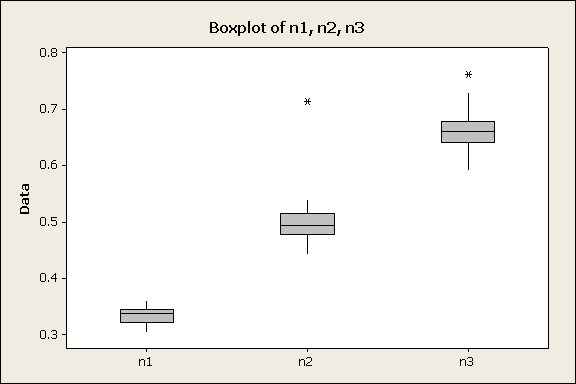
\includegraphics[scale=0.50]{n1n2n3.png}
\caption{Normal distribution}
\label{n1-3}
\end{figure}

\begin{figure}[htp]
\centering
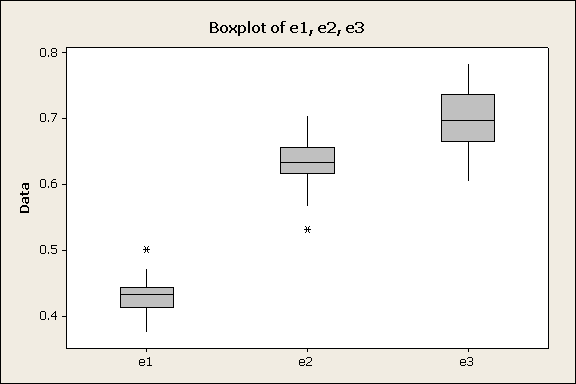
\includegraphics[scale=0.50]{e1e2e3.png}
\caption{Exponential distribution}
\label{e1-3}
\end{figure}

\begin{figure}[htp]
\centering
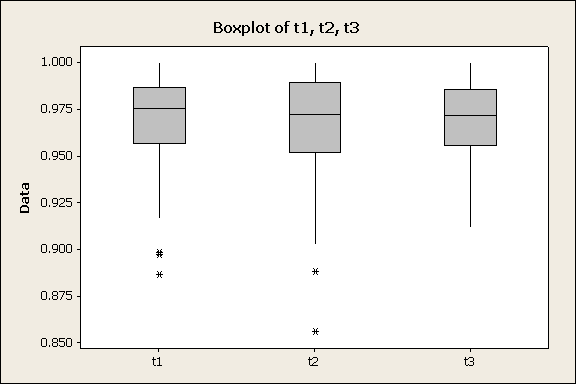
\includegraphics[scale=0.50]{t1t2t3.png}
\caption{Triangular distribution}
\label{t1-3}
\end{figure}

\begin{figure}[htp]
\centering
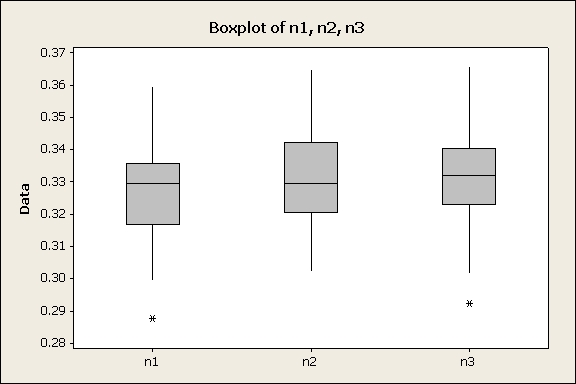
\includegraphics[scale=0.50]{n1n2n3allSame.png}
\caption{Normal distribution, uniform random seed}
\label{n1-3-same}
\end{figure}

\begin{figure}[htp]
\centering
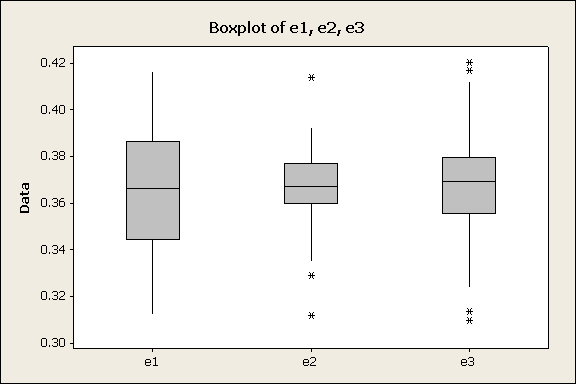
\includegraphics[scale=0.50]{e1e2e3allSame.png}
\caption{Exponential distribution, uniform random seed}
\label{e1-3-same}
\end{figure}

\begin{figure}[htp]
\centering
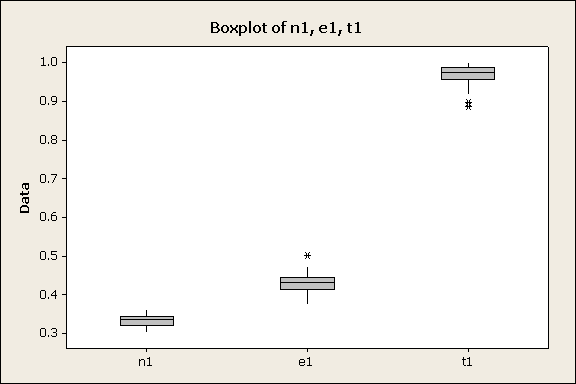
\includegraphics[scale=0.50]{n1e1t1.png}
\caption{First data run across distributions}
\label{n-t1}
\end{figure}

\begin{figure}[htp]
\centering
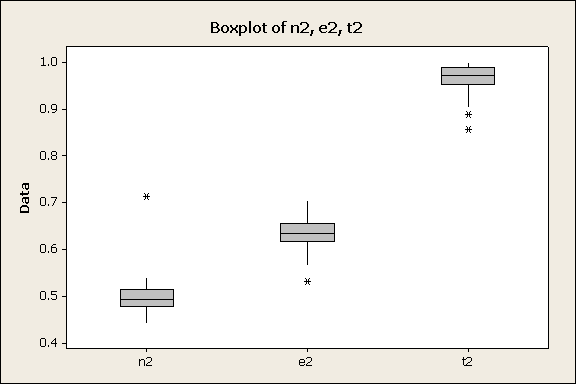
\includegraphics[scale=0.50]{n2e2t2.png}
\caption{Second data run across distributions}
\label{n-t2}
\end{figure}

\begin{figure}[htp]
\centering
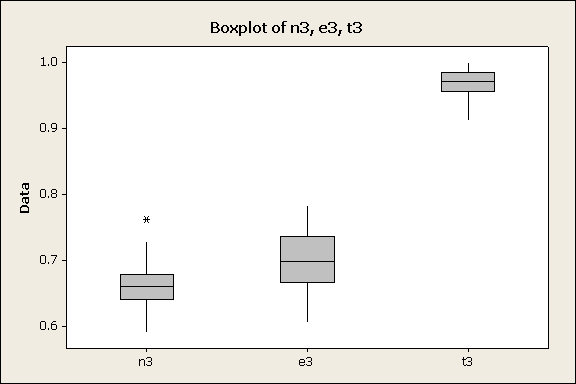
\includegraphics[scale=0.50]{n3e3t3.png}
\caption{Third data run across distributions}
\label{n-t3}
\end{figure}

\end{document}